The feedback current amplifier in Fig \ref{fig:ee18btech11038_probfig} utilizes two identical NMOS transistor sized so that at $I_{D1} = 0.2mA$, they operate at $V_{OV} = 0.2V$. Both the devices have $V_{t} =0.5V$ and $V_{A} = 10V$.




a) If $I_{S}$ has zero DC component, show that both $Q_{1}$ and $Q_{2}$ are, operating at $I_{D} = 0.2mA$. What is DC voltage at the input?
\\
b)Find $g_{m}$ and $r_{o}$ for each $Q_{1}$ and $Q_{2}$.
\\
c) Find the open loop circuit and the value of $R_{i}$, $G$ and $R_{o}$.
\\
d) Find the value of $H$.
\\
e) Find $GH$ and $T$
\\
f)Find $R_{in}$ and $R_{out}$.
\renewcommand{\thefigure}{\theenumi.\arabic{figure}}
\begin{figure}[!ht]
	\begin{center}
		
		\resizebox{\columnwidth}{!}{\begin{circuitikz}[american]
\ctikzset{tripoles/mos style/arrows}
\draw  (0,0) node[ground](GND){} -- (0,1) to[isource, l= $I_{s}$] (0,3) -- (3,3) to[R=$R_{2}(14k\ohm$)] (4,3) -- (6,3)node{} to[R=$R_{1}(3.5k\ohm)$] (6,0) node[ground](GND){} (6,0);

\draw (3,6) node[nmos,](Q1){};
\draw (2,3) node[label={below:A}]{} to[short] (Q1.G);
\draw (Q1.center) node[right]{{$Q_{1}$}};
\draw (Q1.S) -- (3,5) node[ground](GND){};
\draw (3,9) node[vcc](VCC){} to [isource, l =$I(0.2mA)$ ](Q1.D);


\draw (6,7)node[nmos,](Q2){};
\draw (Q2.S) -- (6,3);
\draw (Q2.G) -- (3,7);
\draw (Q2.center) node[right]{{$Q_{2}$}};
\draw (6,9) node[vcc](VCC){} -- (Q2.D);
\draw (1,1)node[label = {below:$R_{in}$}]{} --(1,2);
\draw (1,2) to node[flowarrow]{}(2,2);

\draw (6.5,9.5) ++(0,0.001) node[flowarrow, rotate=-90]{\rotatebox{90}{$I_0$}};
\draw (7,8.7)node[label = {right:$R_{out}$}]{} --(6.5,8.7);
\draw (6.5,8.5) ++(0,-0.1) node[flowarrow, rotate=-90]{};
\end{circuitikz}}
	\end{center}
\caption{Problem Figure}
\label{fig:ee18btech11038_probfig}
\end{figure}

\begin{table}[!ht]
\centering
%%%%%%%%%%%%%%%%%%%%%%%%%%%%%%%%%%%%%%%%%%%%%%%%%%%%%%%%%%%%%%%%%%%%%%
%%                                                                  %%
%%  This is the header of a LaTeX2e file exported from Gnumeric.    %%
%%                                                                  %%
%%  This file can be compiled as it stands or included in another   %%
%%  LaTeX document. The table is based on the longtable package so  %%
%%  the longtable options (headers, footers...) can be set in the   %%
%%  preamble section below (see PRAMBLE).                           %%
%%                                                                  %%
%%  To include the file in another, the following two lines must be %%
%%  in the including file:                                          %%
%%        \def\inputGnumericTable{}                                 %%
%%  at the beginning of the file and:                               %%
%%        \input{name-of-this-file.tex}                             %%
%%  where the table is to be placed. Note also that the including   %%
%%  file must use the following packages for the table to be        %%
%%  rendered correctly:                                             %%
%%    \usepackage[latin1]{inputenc}                                 %%
%%    \usepackage{color}                                            %%
%%    \usepackage{array}                                            %%
%%    \usepackage{longtable}                                        %%
%%    \usepackage{calc}                                             %%
%%    \usepackage{multirow}                                         %%
%%    \usepackage{hhline}                                           %%
%%    \usepackage{ifthen}                                           %%
%%  optionally (for landscape tables embedded in another document): %%
%%    \usepackage{lscape}                                           %%
%%                                                                  %%
%%%%%%%%%%%%%%%%%%%%%%%%%%%%%%%%%%%%%%%%%%%%%%%%%%%%%%%%%%%%%%%%%%%%%%

 

%%  This section checks if we are begin input into another file or  %%
%%  the file will be compiled alone. First use a macro taken from   %%
%%  the TeXbook ex 7.7 (suggestion of Han-Wen Nienhuys).            %%
\def\ifundefined#1{\expandafter\ifx\csname#1\endcsname\relax}


%%  Check for the \def token for inputed files. If it is not        %%
%%  defined, the file will be processed as a standalone and the     %%
%%  preamble will be used.                                          %%
\ifundefined{inputGnumericTable}

%%  We must be able to close or not the document at the end.        %%
	\def\gnumericTableEnd{\end{document}}


%%%%%%%%%%%%%%%%%%%%%%%%%%%%%%%%%%%%%%%%%%%%%%%%%%%%%%%%%%%%%%%%%%%%%%
%%                                                                  %%
%%  This is the PREAMBLE. Change these values to get the right      %%
%%  paper size and other niceties.                                  %%
%%                                                                  %%
%%%%%%%%%%%%%%%%%%%%%%%%%%%%%%%%%%%%%%%%%%%%%%%%%%%%%%%%%%%%%%%%%%%%%%

	\documentclass[12pt%
			  %,landscape%
                    ]{report}
       \usepackage[latin1]{inputenc}
       \usepackage{fullpage}
       \usepackage{color}
       \usepackage{array}
       \usepackage{longtable}
       \usepackage{calc}
       \usepackage{multirow}
       \usepackage{hhline}
       \usepackage{ifthen}

	


%%  End of the preamble for the standalone. The next section is for %%
%%  documents which are included into other LaTeX2e files.          %%
\else

%%  We are not a stand alone document. For a regular table, we will %%
%%  have no preamble and only define the closing to mean nothing.   %%
    \def\gnumericTableEnd{}

%%  If we want landscape mode in an embedded document, comment out  %%
%%  the line above and uncomment the two below. The table will      %%
%%  begin on a new page and run in landscape mode.                  %%
%       \def\gnumericTableEnd{\end{landscape}}
%       \begin{landscape}


%%  End of the else clause for this file being \input.              %%
\fi

%%%%%%%%%%%%%%%%%%%%%%%%%%%%%%%%%%%%%%%%%%%%%%%%%%%%%%%%%%%%%%%%%%%%%%
%%                                                                  %%
%%  The rest is the gnumeric table, except for the closing          %%
%%  statement. Changes below will alter the table's appearance.     %%
%%                                                                  %%
%%%%%%%%%%%%%%%%%%%%%%%%%%%%%%%%%%%%%%%%%%%%%%%%%%%%%%%%%%%%%%%%%%%%%%

\providecommand{\gnumericmathit}[1]{#1} 
%%  Uncomment the next line if you would like your numbers to be in %%
%%  italics if they are italizised in the gnumeric table.           %%
%\renewcommand{\gnumericmathit}[1]{\mathit{#1}}
\providecommand{\gnumericPB}[1]%
{\let\gnumericTemp=\\#1\let\\=\gnumericTemp\hspace{0pt}}
 \ifundefined{gnumericTableWidthDefined}
        \newlength{\gnumericTableWidth}
        \newlength{\gnumericTableWidthComplete}
        \newlength{\gnumericMultiRowLength}
        \global\def\gnumericTableWidthDefined{}
 \fi
%% The following setting protects this code from babel shorthands.  %%
 \ifthenelse{\isundefined{\languageshorthands}}{}{\languageshorthands{english}}
%%  The default table format retains the relative column widths of  %%
%%  gnumeric. They can easily be changed to c, r or l. In that case %%
%%  you may want to comment out the next line and uncomment the one %%
%%  thereafter                                                      %%
\providecommand\gnumbox{\makebox[0pt]}
%%\providecommand\gnumbox[1][]{\makebox}

%% to adjust positions in multirow situations                       %%
\setlength{\bigstrutjot}{\jot}
\setlength{\extrarowheight}{\doublerulesep}

%%  The \setlongtables command keeps column widths the same across  %%
%%  pages. Simply comment out next line for varying column widths.  %%
\setlongtables

\setlength\gnumericTableWidth{%
	83pt+%
	91pt+%
0pt}
\def\gumericNumCols{2}
\setlength\gnumericTableWidthComplete{\gnumericTableWidth+%
         \tabcolsep*\gumericNumCols*2+\arrayrulewidth*\gumericNumCols}
\ifthenelse{\lengthtest{\gnumericTableWidthComplete > \linewidth}}%
         {\def\gnumericScale{\ratio{\linewidth-%
                        \tabcolsep*\gumericNumCols*2-%
                        \arrayrulewidth*\gumericNumCols}%
{\gnumericTableWidth}}}%
{\def\gnumericScale{1}}

%%%%%%%%%%%%%%%%%%%%%%%%%%%%%%%%%%%%%%%%%%%%%%%%%%%%%%%%%%%%%%%%%%%%%%
%%                                                                  %%
%% The following are the widths of the various columns. We are      %%
%% defining them here because then they are easier to change.       %%
%% Depending on the cell formats we may use them more than once.    %%
%%                                                                  %%
%%%%%%%%%%%%%%%%%%%%%%%%%%%%%%%%%%%%%%%%%%%%%%%%%%%%%%%%%%%%%%%%%%%%%%

\ifthenelse{\isundefined{\gnumericColA}}{\newlength{\gnumericColA}}{}\settowidth{\gnumericColA}{\begin{tabular}{@{}p{83pt*\gnumericScale}@{}}x\end{tabular}}
\ifthenelse{\isundefined{\gnumericColB}}{\newlength{\gnumericColB}}{}\settowidth{\gnumericColB}{\begin{tabular}{@{}p{91pt*\gnumericScale}@{}}x\end{tabular}}

\begin{tabular}[c]{%
	b{\gnumericColA}%
	b{\gnumericColB}%
	}

%%%%%%%%%%%%%%%%%%%%%%%%%%%%%%%%%%%%%%%%%%%%%%%%%%%%%%%%%%%%%%%%%%%%%%
%%  The longtable options. (Caption, headers... see Goosens, p.124) %%
%	\caption{The Table Caption.}             \\	%
% \hline	% Across the top of the table.
%%  The rest of these options are table rows which are placed on    %%
%%  the first, last or every page. Use \multicolumn if you want.    %%

%%  Header for the first page.                                      %%
%	\multicolumn{2}{c}{The First Header} \\ \hline 
%	\multicolumn{1}{c}{colTag}	%Column 1
%	&\multicolumn{1}{c}{colTag}	\\ \hline %Last column
%	\endfirsthead

%%  The running header definition.                                  %%
%	\hline
%	\multicolumn{2}{l}{\ldots\small\slshape continued} \\ \hline
%	\multicolumn{1}{c}{colTag}	%Column 1
%	&\multicolumn{1}{c}{colTag}	\\ \hline %Last column
%	\endhead

%%  The running footer definition.                                  %%
%	\hline
%	\multicolumn{2}{r}{\small\slshape continued\ldots} \\
%	\endfoot

%%  The ending footer definition.                                   %%
%	\multicolumn{2}{c}{That's all folks} \\ \hline 
%	\endlastfoot
%%%%%%%%%%%%%%%%%%%%%%%%%%%%%%%%%%%%%%%%%%%%%%%%%%%%%%%%%%%%%%%%%%%%%%

\hhline{|-|-}
	 \multicolumn{1}{|p{\gnumericColA}|}%
	{\gnumericPB{\raggedright}\gnumbox[l]{\textbf{Parameter}}}
	&\multicolumn{1}{p{\gnumericColA}|}%
	{\gnumericPB{\raggedright}\gnumbox[l]{\textbf{Value}}}
\\
\hhline{|-|-}
	 \multicolumn{1}{|p{\gnumericColA}|}%
	{\gnumericPB{\raggedright}\gnumbox[l]{\textbf{$R_{1}$}}}
	&\multicolumn{1}{p{\gnumericColA}|}%
	{\gnumericPB{\raggedright}\gnumbox[l]{\textbf{$3.5k\Omega$}}}
\\
\hhline{|-|-}
	 \multicolumn{1}{|p{\gnumericColA}|}%
	{\gnumericPB{\raggedright}\gnumbox[l]{\textbf{$R_{2}$}}}
	&\multicolumn{1}{p{\gnumericColA}|}%
	{\gnumericPB{\raggedright}\gnumbox[l]{\textbf{$14k\Omega$}}}
\\
\hhline{|-|-}
	 \multicolumn{1}{|p{\gnumericColA}|}%
	{\gnumericPB{\raggedright}\gnumbox[l]{\textbf{$I_{D1}$}}}
	&\multicolumn{1}{p{\gnumericColA}|}%
	{\gnumericPB{\raggedright}\gnumbox[l]{\textbf{$0.2mA$}}}
\\
\hhline{|-|-}
	 \multicolumn{1}{|p{\gnumericColA}|}%
	{\gnumericPB{\raggedright}\gnumbox[l]{\textbf{$V_{OV}$}}}
	&\multicolumn{1}{p{\gnumericColA}|}%
	{\gnumericPB{\raggedright}\gnumbox[l]{\textbf{$0.2V$}}}

\\
\hhline{|-|-}
	 \multicolumn{1}{|p{\gnumericColA}|}%
	{\gnumericPB{\raggedright}\gnumbox[l]{\textbf{$V_{t}$}}}
	&\multicolumn{1}{p{\gnumericColA}|}%
	{\gnumericPB{\raggedright}\gnumbox[l]{\textbf{$0.5V$}}}
\\
\hhline{|-|-}
	 \multicolumn{1}{|p{\gnumericColA}|}%
	{\gnumericPB{\raggedright}\gnumbox[l]{\textbf{$V_{A}$}}}
	&\multicolumn{1}{p{\gnumericColA}|}%
	{\gnumericPB{\raggedright}\gnumbox[l]{\textbf{$10V$}}}

\\

\hhline{|-|-|}
\end{tabular}

\ifthenelse{\isundefined{\languageshorthands}}{}{\languageshorthands{\languagename}}
\gnumericTableEnd
\caption{Given Parameters}
\label{table: given}
\end{table}

\begin{enumerate}[label=\arabic*.,ref=\theenumi]
\numberwithin{equation}{enumi}
\renewcommand{\thefigure}{\theenumi.\arabic{figure}}
\item a)DC analysis of circuit.\\
\solution Given that $I_{s}$ has zero DC component, it can be neglected in DC analysis of the circuit. The current does not enter the Gate terminal of any mosfet. Thus the DC current flow looks like shown in Fig \ref{fig:ee18btech11038_dcckt} 

\begin{figure}[!ht]
	\begin{center}
		
		\resizebox{\columnwidth}{!}{\begin{circuitikz}[american]
\ctikzset{tripoles/mos style/arrows}
\draw (2,3) to[R=$R_{2}(14k\ohm$), i=$I_{dc}(0)$] (6,3) -- (6,3)node{} to[R=$R_{1}(3.5k\ohm)$] (6,0) node[ground](GND){} (6,0);

\draw (3,6) node[nmos,](Q1){};
\draw (2,3) node[]{} to[short] (Q1.G);
\draw (Q1.center) node[right]{{$Q_{1}$}};
\draw (Q1.S) to[short, i=$I_{D1}$](3, 5) -- (3,5) node[ground](GND){};
\draw (3,9) node[vcc](VCC){} to[short, i=$I_{D1}$](3,8.5) to[isource, l =$I(0.2mA)$ ](Q1.D);


\draw (6,7)node[nmos,](Q2){};
\draw (Q2.S) to[short, i=$I_{D2}$](6, 3) -- (6,3);
\draw (Q2.G) -- (3,7);
\draw (Q2.center) node[right]{{$Q_{2}$}};
\draw (6,9) node[vcc](VCC){} to[short, i=$I_{D2}$](6,8.5) -- (Q2.D);
\draw (2,3) to[short, -o] (2,2.5)node[below]{$V_{G1}$};
\draw (5,7) to[short, -o] (5,6.5)node[below]{$V_{G2}$};
\draw (6,3) to[short, -o] (6.5,3)node[right]{$V_{S2}$};
\draw (3,7) to[short, -o] (2.5,7)node[left]{$V_{D2}$};
\end{circuitikz}}
	\end{center}
\caption{DC Analysis Circuit}
\label{fig:ee18btech11038_dcckt}
\end{figure}

Given $V_{OV} = 0.2V$ and  $V_{t} = 0.5V$, for Q1-
\begin{align}
    V_{GS1} = V_{OV}  + V_{t} = 0.7V\\
    \implies V_{G1} = V_{GS1} = 0.7V
    \end{align}
\begin{align}
    \text{The DC voltage } V_{G1} = V_{S2}\\
    \text{by ohms law, } I_{D2} = \frac{V_{S2}}{R{1}} = \frac{0.7V}{3.5k\ohm}\\
    \implies I_{D2} = 0.2mA
\end{align}
Clearly $I_{D1} = 0.2mA$.
\\
DC voltage at input = $V_{G1} = 0.7V$

\item Verify the DC values $I_{D2}$ and $V_{G1}$.\\
\solution Simulate the circuit, Fig \ref{fig:ee18btech11038_dcckt}, using spice. Observe the DC operating point values. Fig \ref{fig:ee18btech11038_dc} shows that $I_{D2}$ is close to 0.2mA and $V_{G1}$ is close to 0.7V.
You can find the netlist for the simulated circuit here:
\begin{lstlisting}
spice/ee18btech11038_dc.cir
\end{lstlisting}
You can find the python script used to generate the output here:
\begin{lstlisting}
spice/ee18btech11038_dc.py
\end{lstlisting}

\begin{figure}[!ht]
\centering
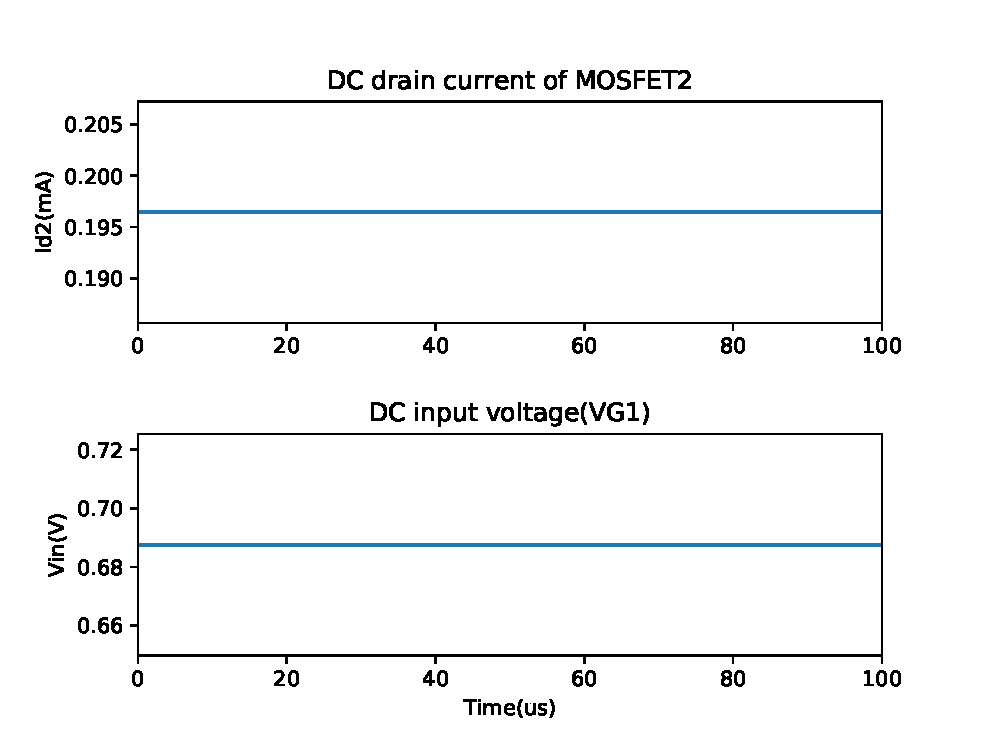
\includegraphics[width=\columnwidth]{./figs/ee18btech11038_dc.eps}
\caption{Simulation for Verifying DC operating point}
\label{fig:ee18btech11038_dc}
\end{figure}


\item To find $g_{m}$ and $r_{o}$\\
\solution We know,
\begin{align}
    \text{transconductance, } g_{m} = \frac{2I_{D}}{V_{OV}} 
\end{align}
therefore-
\begin{align}
    g_{m1} = g_{m2} = \frac{(2)(0.2)(10^-3)}{0.2}\\
    \implies 2mA/V
\end{align}
$r_{o}$ is given by,
\begin{align}
    r_{0} = \frac{V_{A}}{I_{D}}\\
    \implies r_{o1} = r_{o2} = 50k\ohm
\end{align}

\item c) To find open loop circuit.\\
\solution The general open loop circuit for a current(series-shunt) amplifier is shown in Fig \ref{fig:ee18btech11038_genamp}.

\begin{figure}[!ht]
	\begin{center}
		
		\resizebox{\columnwidth}{!}{\begin{circuitikz}[american]
\tikzset{quad/.style={draw, minimum height=2.4cm, minimum width=4cm}}
\node[quad] (A) at (0,0) {$Basic\quad Amp$};
\draw ($(A.north west)!.175!(A.west)$) to[short] ++(-3,0)
      ($(A.south west)!.175!(A.west)$) to[short] ++(-3,0)
      ($(A.north east)!.175!(A.east)$) to[short] ++(1,0)
      ($(A.south east)!.175!(A.east)$) to[short] ++(1,0);

\draw (-4,-1) to[R,n=res1] (-4,1);
\draw (-5,-1) -- (-6,-1);
\draw (-5,1) -- (-6,1);
\draw (-6,-1) -- (-7.5,-1) to[isource, l= $I_{i}$] (-7.5,1) -- (-6,1);
\draw (-6,-1) to[R,n=res3] (-6,1);
\draw (3,-1) to[R,n=res2] (5,-1) -- (6,-1) to[R=$R_{L}$] (6,1) -- (3,1);
\draw (res1.s) node[right]{$R_{11}$};
\draw (res3.s) node[right]{$R_{s}$};
\draw (res2.s) node[below]{$R_{22}$};

\end{circuitikz}}
	\end{center}
\caption{General open loop circuit}
\label{fig:ee18btech11038_genamp}
\end{figure}

\begin{table}[!ht]
\centering
%%%%%%%%%%%%%%%%%%%%%%%%%%%%%%%%%%%%%%%%%%%%%%%%%%%%%%%%%%%%%%%%%%%%%%
%%                                                                  %%
%%  This is the header of a LaTeX2e file exported from Gnumeric.    %%
%%                                                                  %%
%%  This file can be compiled as it stands or included in another   %%
%%  LaTeX document. The table is based on the longtable package so  %%
%%  the longtable options (headers, footers...) can be set in the   %%
%%  preamble section below (see PRAMBLE).                           %%
%%                                                                  %%
%%  To include the file in another, the following two lines must be %%
%%  in the including file:                                          %%
%%        \def\inputGnumericTable{}                                 %%
%%  at the beginning of the file and:                               %%
%%        \input{name-of-this-file.tex}                             %%
%%  where the table is to be placed. Note also that the including   %%
%%  file must use the following packages for the table to be        %%
%%  rendered correctly:                                             %%
%%    \usepackage[latin1]{inputenc}                                 %%
%%    \usepackage{color}                                            %%
%%    \usepackage{array}                                            %%
%%    \usepackage{longtable}                                        %%
%%    \usepackage{calc}                                             %%
%%    \usepackage{multirow}                                         %%
%%    \usepackage{hhline}                                           %%
%%    \usepackage{ifthen}                                           %%
%%  optionally (for landscape tables embedded in another document): %%
%%    \usepackage{lscape}                                           %%
%%                                                                  %%
%%%%%%%%%%%%%%%%%%%%%%%%%%%%%%%%%%%%%%%%%%%%%%%%%%%%%%%%%%%%%%%%%%%%%%



%%  This section checks if we are begin input into another file or  %%
%%  the file will be compiled alone. First use a macro taken from   %%
%%  the TeXbook ex 7.7 (suggestion of Han-Wen Nienhuys).            %%
\def\ifundefined#1{\expandafter\ifx\csname#1\endcsname\relax}


%%  Check for the \def token for inputed files. If it is not        %%
%%  defined, the file will be processed as a standalone and the     %%
%%  preamble will be used.                                          %%
\ifundefined{inputGnumericTable}

%%  We must be able to close or not the document at the end.        %%
	\def\gnumericTableEnd{\end{document}}


%%%%%%%%%%%%%%%%%%%%%%%%%%%%%%%%%%%%%%%%%%%%%%%%%%%%%%%%%%%%%%%%%%%%%%
%%                                                                  %%
%%  This is the PREAMBLE. Change these values to get the right      %%
%%  paper size and other niceties.                                  %%
%%                                                                  %%
%%%%%%%%%%%%%%%%%%%%%%%%%%%%%%%%%%%%%%%%%%%%%%%%%%%%%%%%%%%%%%%%%%%%%%

	\documentclass[12pt%
			  %,landscape%
                    ]{report}
       \usepackage[latin1]{inputenc}
       \usepackage{fullpage}
       \usepackage{color}
       \usepackage{array}
       \usepackage{longtable}
       \usepackage{calc}
       \usepackage{multirow}
       \usepackage{hhline}
       \usepackage{ifthen}

	\begin{document}


%%  End of the preamble for the standalone. The next section is for %%
%%  documents which are included into other LaTeX2e files.          %%
\else

%%  We are not a stand alone document. For a regular table, we will %%
%%  have no preamble and only define the closing to mean nothing.   %%
    \def\gnumericTableEnd{}

%%  If we want landscape mode in an embedded document, comment out  %%
%%  the line above and uncomment the two below. The table will      %%
%%  begin on a new page and run in landscape mode.                  %%
%       \def\gnumericTableEnd{\end{landscape}}
%       \begin{landscape}


%%  End of the else clause for this file being \input.              %%
\fi

%%%%%%%%%%%%%%%%%%%%%%%%%%%%%%%%%%%%%%%%%%%%%%%%%%%%%%%%%%%%%%%%%%%%%%
%%                                                                  %%
%%  The rest is the gnumeric table, except for the closing          %%
%%  statement. Changes below will alter the table's appearance.     %%
%%                                                                  %%
%%%%%%%%%%%%%%%%%%%%%%%%%%%%%%%%%%%%%%%%%%%%%%%%%%%%%%%%%%%%%%%%%%%%%%

\providecommand{\gnumericmathit}[1]{#1} 
%%  Uncomment the next line if you would like your numbers to be in %%
%%  italics if they are italizised in the gnumeric table.           %%
%\renewcommand{\gnumericmathit}[1]{\mathit{#1}}
\providecommand{\gnumericPB}[1]%
{\let\gnumericTemp=\\#1\let\\=\gnumericTemp\hspace{0pt}}
 \ifundefined{gnumericTableWidthDefined}
        \newlength{\gnumericTableWidth}
        \newlength{\gnumericTableWidthComplete}
        \newlength{\gnumericMultiRowLength}
        \global\def\gnumericTableWidthDefined{}
 \fi
%% The following setting protects this code from babel shorthands.  %%
 \ifthenelse{\isundefined{\languageshorthands}}{}{\languageshorthands{english}}
%%  The default table format retains the relative column widths of  %%
%%  gnumeric. They can easily be changed to c, r or l. In that case %%
%%  you may want to comment out the next line and uncomment the one %%
%%  thereafter                                                      %%
\providecommand\gnumbox{\makebox[0pt]}
%%\providecommand\gnumbox[1][]{\makebox}

%% to adjust positions in multirow situations                       %%
\setlength{\bigstrutjot}{\jot}
\setlength{\extrarowheight}{\doublerulesep}

%%  The \setlongtables command keeps column widths the same across  %%
%%  pages. Simply comment out next line for varying column widths.  %%
\setlongtables

\setlength\gnumericTableWidth{%
	53pt+%
	163pt+%
0pt}
\def\gumericNumCols{2}
\setlength\gnumericTableWidthComplete{\gnumericTableWidth+%
         \tabcolsep*\gumericNumCols*2+\arrayrulewidth*\gumericNumCols}
\ifthenelse{\lengthtest{\gnumericTableWidthComplete > \linewidth}}%
         {\def\gnumericScale{\ratio{\linewidth-%
                        \tabcolsep*\gumericNumCols*2-%
                        \arrayrulewidth*\gumericNumCols}%
{\gnumericTableWidth}}}%
{\def\gnumericScale{1}}

%%%%%%%%%%%%%%%%%%%%%%%%%%%%%%%%%%%%%%%%%%%%%%%%%%%%%%%%%%%%%%%%%%%%%%
%%                                                                  %%
%% The following are the widths of the various columns. We are      %%
%% defining them here because then they are easier to change.       %%
%% Depending on the cell formats we may use them more than once.    %%
%%                                                                  %%
%%%%%%%%%%%%%%%%%%%%%%%%%%%%%%%%%%%%%%%%%%%%%%%%%%%%%%%%%%%%%%%%%%%%%%

\ifthenelse{\isundefined{\gnumericColA}}{\newlength{\gnumericColA}}{}\settowidth{\gnumericColA}{\begin{tabular}{@{}p{53pt*\gnumericScale}@{}}x\end{tabular}}
\ifthenelse{\isundefined{\gnumericColB}}{\newlength{\gnumericColB}}{}\settowidth{\gnumericColB}{\begin{tabular}{@{}p{163pt*\gnumericScale}@{}}x\end{tabular}}

\begin{tabular}[c]{%
	b{\gnumericColA}%
	b{\gnumericColB}%
	}

%%%%%%%%%%%%%%%%%%%%%%%%%%%%%%%%%%%%%%%%%%%%%%%%%%%%%%%%%%%%%%%%%%%%%%
%%  The longtable options. (Caption, headers... see Goosens, p.124) %%
%	\caption{The Table Caption.}             \\	%
% \hline	% Across the top of the table.
%%  The rest of these options are table rows which are placed on    %%
%%  the first, last or every page. Use \multicolumn if you want.    %%

%%  Header for the first page.                                      %%
%	\multicolumn{2}{c}{The First Header} \\ \hline 
%	\multicolumn{1}{c}{colTag}	%Column 1
%	&\multicolumn{1}{c}{colTag}	\\ \hline %Last column
%	\endfirsthead

%%  The running header definition.                                  %%
%	\hline
%	\multicolumn{2}{l}{\ldots\small\slshape continued} \\ \hline
%	\multicolumn{1}{c}{colTag}	%Column 1
%	&\multicolumn{1}{c}{colTag}	\\ \hline %Last column
%	\endhead

%%  The running footer definition.                                  %%
%	\hline
%	\multicolumn{2}{r}{\small\slshape continued\ldots} \\
%	\endfoot

%%  The ending footer definition.                                   %%
%	\multicolumn{2}{c}{That's all folks} \\ \hline 
%	\endlastfoot
%%%%%%%%%%%%%%%%%%%%%%%%%%%%%%%%%%%%%%%%%%%%%%%%%%%%%%%%%%%%%%%%%%%%%%

\hhline{|-|-}
	 \multicolumn{1}{|p{\gnumericColA}|}%
	{\gnumericPB{\centering}\gnumbox{\textbf{Resistance}}}
	&\multicolumn{1}{p{\gnumericColB}|}%
	{\gnumericPB{\centering}\gnumbox{\textbf{Description}}}
\\
\hhline{|--|}
	 \multicolumn{1}{|p{\gnumericColA}|}%
	{\gnumericPB{\raggedright}\gnumbox[l]{$R_{in}$}}
	&\multicolumn{1}{p{\gnumericColB}|}%
	{\gnumericPB{\raggedright}\gnumbox[l]{Total Input Resistance}}
\\
\hhline{|--|}
	 \multicolumn{1}{|p{\gnumericColA}|}%
	{\gnumericPB{\raggedright}\gnumbox[l]{$R_{out}$}}
	&\multicolumn{1}{p{\gnumericColB}|}%
	{\gnumericPB{\raggedright}\gnumbox[l]{Total Ouput Resistance}}
\\
\hhline{|--|}
	 \multicolumn{1}{|p{\gnumericColA}|}%
	{\gnumericPB{\raggedright}\gnumbox[l]{$r_{o1}$}}
	&\multicolumn{1}{p{\gnumericColB}|}%
	{\gnumericPB{\raggedright}\gnumbox[l]{Output resistance of MOSFET1}}
\\
\hhline{|--|}
	 \multicolumn{1}{|p{\gnumericColA}|}%
	{\gnumericPB{\raggedright}\gnumbox[l]{$r_{o2}$}}
	&\multicolumn{1}{p{\gnumericColB}|}%
	{\gnumericPB{\raggedright}\gnumbox[l]{Output resistance of MOSFET2}}
\\
\hhline{|--|}
	 \multicolumn{1}{|p{\gnumericColA}|}%
	{\gnumericPB{\raggedright}\gnumbox[l]{$R_{i}$}}
	&\multicolumn{1}{p{\gnumericColB}|}%
	{\gnumericPB{\raggedright}\gnumbox[l]{Input resistance of Open Loop}}
\\
\hhline{|--|}
	 \multicolumn{1}{|p{\gnumericColA}|}%
	{\gnumericPB{\raggedright}\gnumbox[l]{$R_{o}$}}
	&\multicolumn{1}{p{\gnumericColB}|}%
	{\gnumericPB{\raggedright}\gnumbox[l]{Output resistance of Open Loop}}
\\
\hhline{|--|}
	 \multicolumn{1}{|p{\gnumericColA}|}%
	{\gnumericPB{\raggedright}\gnumbox[l]{$R_{if}$}}
	&\multicolumn{1}{p{\gnumericColB}|}%
	{\gnumericPB{\raggedright}\gnumbox[l]{Input resistance of Feedback}}
\\
\hhline{|--|}
	 \multicolumn{1}{|p{\gnumericColA}|}%
	{\gnumericPB{\raggedright}\gnumbox[l]{$R_{of}$}}
	&\multicolumn{1}{p{\gnumericColB}|}%
	{\gnumericPB{\raggedright}\gnumbox[l]{Output resistance of Feedback}}
\\
\hhline{|--|}
	 \multicolumn{1}{|p{\gnumericColA}|}%
	{\gnumericPB{\raggedright}\gnumbox[l]{$R_{s}$}}
	&\multicolumn{1}{p{\gnumericColB}|}%
	{\gnumericPB{\raggedright}\gnumbox[l]{Resistance of Current Source}}
\\
\hhline{|--|}
	 \multicolumn{1}{|p{\gnumericColA}|}%
	{\gnumericPB{\raggedright}\gnumbox[l]{$R_{L}$}}
	&\multicolumn{1}{p{\gnumericColB}|}%
	{\gnumericPB{\raggedright}\gnumbox[l]{Output Load Resistance}}
\\
\hhline{|--|}
	 \multicolumn{1}{|p{\gnumericColA}|}%
	{\gnumericPB{\raggedright}\gnumbox[l]{$R_{11}$}}
	&\multicolumn{1}{p{\gnumericColB}|}%
	{\gnumericPB{\raggedright}\gnumbox[l]{Input load resist. (due feedback) }}
\\
\hhline{|--|}
	 \multicolumn{1}{|p{\gnumericColA}|}%
	{\gnumericPB{\raggedright}\gnumbox[l]{$R_{22}$}}
	&\multicolumn{1}{p{\gnumericColB}|}%
	{\gnumericPB{\raggedright}\gnumbox[l]{Output load resist. (due feedback)}}
\\
\hhline{|-|-|}
\end{tabular}

\ifthenelse{\isundefined{\languageshorthands}}{}{\languageshorthands{\languagename}}
\gnumericTableEnd
\caption{Resistances}
\label{table: restable}
\end{table}

For our problem, the small circuit model is shown in Fig \ref{fig:ee18btech11038_smlckt}. All the different resistances are summarized in Table \ref{table: restable}

\begin{figure}[!ht]
	\begin{center}
		
		\resizebox{\columnwidth}{!}{\begin{circuitikz}[american]
\ctikzset{tripoles/mos style/arrows}
\draw  (0,0) node[ground](GND){} -- (0,1) to[isource, l= $I_{s}$] (0,3) -- (3,3) to[R=$R_{2}(14k\ohm$), i=$I_{s}$] (6,3) -- (6,3)node{} to[R=$R_{1}(3.5k\ohm)$] (6,0) node[ground](GND){} (6,0);

\draw (3,6) node[nmos,](Q1){};
\draw (2,3)  to[short, i=$i(0)$] (Q1.G);
\draw (Q1.center) node[right]{{$Q_{1}$}};
\draw (Q1.S) -- (3,5) node[ground](GND){};
\draw (Q1.D) -- (3,7);
\draw (3,6.75) -- (4,6.75) to[R= $r_{o1}$](4,5.25) -- (3,5.25);



\draw (6,7)node[nmos,](Q2){};
\draw (Q2.S) to[short, i=$I_{o}$](6, 3) -- (6,3);
\draw (Q2.G) -- (3,7);
\draw (Q2.center) node[right]{{$Q_{2}$}};
\draw (6,9) node[ground, rotate=180]{} to[short, i=$I_{o}$](6,8.5) -- (Q2.D);
\draw (6,7.75) -- (7,7.75) to[R= $r_{o2}$](7,6.25) -- (6,6.25);

\draw (2,1)node[label = {below:$Port 1$}]{} --(2,2);
\draw (2,2) to node[flowarrow]{}(3,2);
\draw (2,3) to[short, -o] (2,2.5)node[below]{$v_{g1}$};
\draw (5,7) to[short, -o] (5,6.5)node[below]{$v_{g2}$};
\draw (6,3) to[short, -o] (6.5,3)node[right]{$v_{s2}$};
\draw (3,7) to[short, -o] (2.5,7)node[left]{$v_{d1}$};
\draw (7,5) ++(0,-0.1) node[flowarrow, rotate=-90]{\rotatebox{90}{$Port 2$}};
\draw[dashed] (3,1) to[short](3,4) to[short](8, 4) to[short](8,1) to[short](3,1);

\end{circuitikz}}
	\end{center}
\caption{Small Circuit Model}
\label{fig:ee18btech11038_smlckt}
\end{figure}



For a shunt-series amplifier, $R_{11}$ is the resistance looking into the feedback circuit from port 1 while port 2 is open circuited.
\begin{align}
    R_{11} = R_{1} + R_{2}
\end{align}

$R_{22}$ is the resistance looking into the feedback circuit from port 2 while port 1 is short circuited.
\begin{align}
    R_{22} = R_{1}||R_{2}
\end{align}

Also for our problem, $R_{L} = 0$ and $R_{s} = \infty$.Open loop circuit for our problem is shown in Fig \ref{fig:ee18btech11038_Ackt}.
\begin{figure}[!ht]
	\begin{center}
		
		\resizebox{\columnwidth}{!}{\begin{circuitikz}[american]
\ctikzset{tripoles/mos style/arrows}
\draw (-6, 0)node[ground]{} to[isource, l= $I_{s}$](-6,4) to[short](-4,4) to[R= $R_{11}$](-4,0) to (-4,0)node[ground]{};
\draw (-4,4) to[short, -o] (-3,4)node[right]{$v_{g1}$};
\draw (-3,4)node[below]{$+$};
\draw (-3,0)node[]{$-$};
\draw (-3, 2)node[]{$v_{g1}$};

\draw (0,0) node[ground]{} to[R=$r_{o1}$](0,2) to[short](0,4) to[short](-2,4) to[cisource, l = $g_{m1}v_{g1}$](-2,0) to (-2,0)node[ground]{};
\draw (0,4) to[short, -o] (1,4)node[right]{$v_{g2}$};
\draw (1,4)node[below]{$+$};
\draw (1,0)node[]{$-$};
\draw (1, 2)node[]{$v_{g2}$};

\draw (5,0)node[below]{$X$} to[R = $r_{o2}$](5,2) to[short](5,4) to [short](5,4) to[short](2,4) to[cisource, l=$g_{m2}(v_{g2} - v_{s2})$](2,0) to[short](5,0);
\draw (2,0) to[short, -o] (2,-0.5)node[below]{$v_{s2}$};
\draw (2,4) to[short] (2,5)node[ground, rotate=180]{};
%\draw (5,4) to[short](7,4) to[short, i= $I_{o}$](7,2) to[short](7,0) to[R=$R_{22}$](5,0);
\draw (7,2) to[short, o-o] (7,1);
\draw (7,2)node[right]{$Y`$};
\draw (7,1)node[right]{$Y$};
\draw (5,0) to[R=$R_{22}$](7,0) to[short](7,2) to[short, i=$I_{o}$](7,4) to[short](5,4);





\end{circuitikz}}
	\end{center}
\caption{Open loop circuit}
\label{fig:ee18btech11038_Ackt}
\end{figure}

From the open loop circuit, Fig \ref{fig:ee18btech11038_Ackt}, we have-
\begin{align}
\label{eq:VG2}
    v_{g1} = I_{s}R_{11} = I_{s}(R_{1} + R_{2})\\
\label{eq:VG@}
    v_{g2} = -g_{m1}v_{g1}r_{o1}\\
    \implies g_{m1}r_{o1}(R_{1} + R_{2})I_{s}
\end{align}
KCL at node X yields -
\begin{align}
    g_{m2}(v_{g2} - v_{s2}) = \frac{v_{s2}}{r_{02}||R_{22}}\\ \\
    \implies g_{m2}v_{g2} = (g_{m2} + \frac{1}{r_{o2}||R_{22}})v_{s2}\\ \\
    \implies v_{s2} = \frac{v_{g2}g_{m2}}{g_{m2} + \frac{1}{r_{02}||R_{22}}}\\
\end{align}
therefore,
\begin{align}
    I_{o} = \frac{v_{s2}}{R_{22}}\\
    \implies \frac{v_{g2}g_{m2}}{g_{m2}(R_{1} + R_{2}) + \frac{R_{1}||R_{2}}{r_{o2}||R_{1}||R_{2}}}
\end{align}
Substituting $v_{g2}$ from \ref{eq:VG@},
\begin{align}
    I_{o} = \frac{-g_{m1}g_{m2}r_{o1}(R_{1} + R_{2})I_{s}}{g_{m2}(R_{1}||R_{2}) + \frac{R_{1}||R_{2}}{r_{o2}||R_{1}||R_{2}}}
\end{align}
Thus, open loop gain G- 
\begin{align}
    G = \frac{I_{o}}{I_{s}}\\
    \implies \frac{-g_{m1}g_{m2}r_{o1}(R_{1} + R_{2})}{g_{m2}(R_{1}||R_{2}) + \frac{R_{1}||R_{2}}{r_{o2}||R_{1}||R_{2}}}
\end{align}
\item Verify the open loop gain value($G$).\\
\solution Simulate the circuit, Fig \ref{fig:ee18btech11038_Ackt}, using spice. Pass small signal as input $I_{s}$ and observe the output. 
Fig \ref{fig:ee18btech11038_olgain} shows that $G = -525.76$ which is closed to that obtained in Table \ref{table: finalvalues}.
You can find the netlist for the simulated circuit here:
\begin{lstlisting}
spice/ee18btech11038_olgain.cir
\end{lstlisting}
You can find the python script used to generate the output here:
\begin{lstlisting}
spice/ee18btech11038_olgain.py
\end{lstlisting}

\begin{figure}[!ht]
\centering
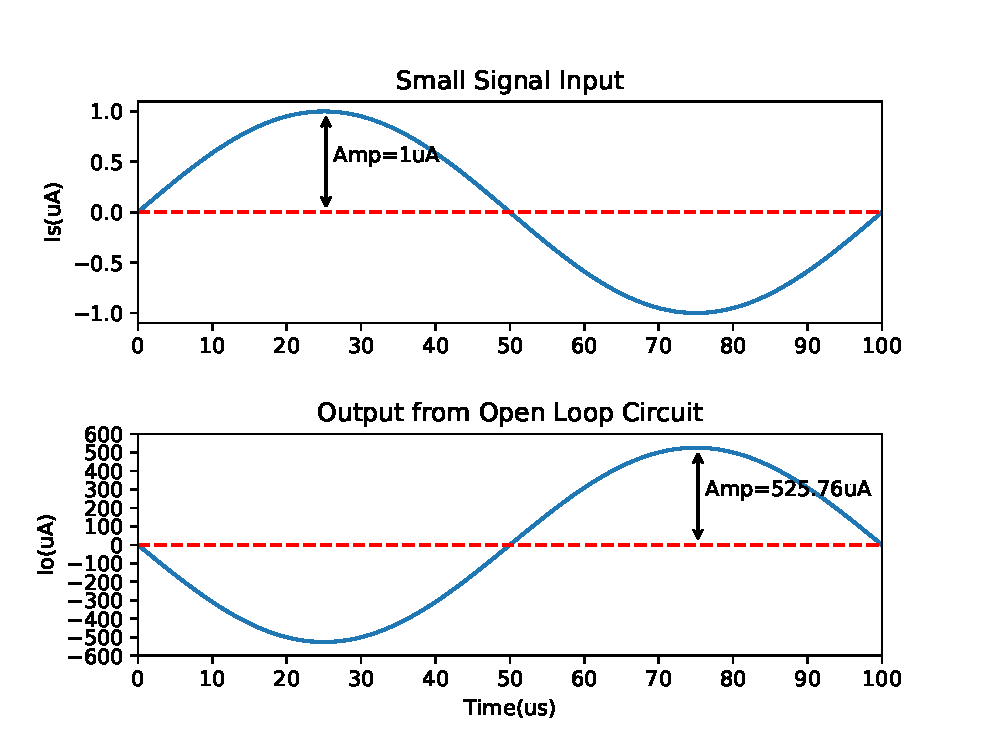
\includegraphics[width=\columnwidth]{./figs/ee18btech11038_olgain.eps}
\caption{Simulation for Open loop gain}
\label{fig:ee18btech11038_olgain}
\end{figure}

\item c)Input Resistance for Open loop\\
\solution Input resistance of the Open loop, $R_{i}$, see Fig \ref{fig:ee18btech11038_Ackt}, clearly is-
\begin{align}
\label{eq:Ri}
    R_{i} = R_{1} + R_{2}
\end{align}
\item c) To find Output Resistance of Open loop, $R_{o}$\\
\solution See Fig \ref{fig:ee18btech11038_outckt} which is the output circuit obtained by breaking the open loop circuit, Fig \ref{fig:ee18btech11038_Ackt}, at YY` and setting the input to zero. $R_{o}$ is the resistance looking into YY`.

\begin{figure}[!ht]
	\begin{center}
		
		\resizebox{\columnwidth}{!}{\begin{circuitikz}[american]
\ctikzset{tripoles/mos style/arrows}
\draw (0,0)node[ground]{} to[R=$R_{22}$](0,1) to[short](0,3) to[short](3,3) to[R=$r_{o2}$](3,6) to[short](0,6) to[cisource, l=$g_{m2}v_{gs2}$](0,3);
\draw (0,3) to[short, -o] (-2,3)node[above]{$-v_{gs2}$};
\draw (-2,0)node[below]{$+$};
\draw (-2,3)node[below]{$-$};
\draw (-2, 1.5)node[]{$v_{gs2}$};
\draw (6,0)node[ground]{} to[vsource, l=$V_{x}$](6,6) to[short](3,6);
\end{circuitikz}}
	\end{center}
\caption{Output Circuit}
\label{fig:ee18btech11038_outckt}
\end{figure}

The current source can be changed into an equivalent voltage source, and the circuit obtained is Fig \ref{fig:ee18btech11038_simpout}.
\begin{figure}[!ht]
	\begin{center}
		
		\resizebox{\columnwidth}{!}{\begin{circuitikz}[american]
\ctikzset{tripoles/mos style/arrows}
\draw (0,0)node[ground]{} to[R=$R_{22}$](0,1) to[short](0,3);
\draw (0,3) to[short, -o] (-2,3)node[above]{$-v_{gs2}$};
\draw (-2,0)node[below]{$+$};
\draw (-2,3)node[below]{$-$};
\draw (-2,1.5)node[]{$v_{gs2}$};
\draw (3,4)node[ground]{} to[vsource, l=$V_{x}$](3,7) to[short, i=$I_{x}$](0,7) to[R=$r_{o2}$](0,5) to[vsource, l=$g_{m2}v_{gs2}$](0,3);

\end{circuitikz}}
	\end{center}
\caption{Simplified Output Circuit}
\label{fig:ee18btech11038_simpout}
\end{figure}

From circuit Fig \ref{fig:ee18btech11038_simpout}, we have,
\begin{align}
\label{eq:fsteqn}
    v_{gs2} = -I_{x}R_{22}\\
\label{eq:seceqn}
    v_{x} + g_{m2}v_{gs2}r_{o2} = I_{x}(r_{o2} + R_{22})
\end{align}
On subtituting \ref{eq:fsteqn} in \ref{eq:seceqn} and simplifying, we get,
\begin{align}
    \frac{v_{x}}{I_{x}} = r_{o2} + R_{22} + g_{m2}r_{o2}R_{22}\\
\label{eq:Ro}
    \implies R_{o} =r_{o2} + R_{1}||R_{2} + g_{m2}r_{o2}(R_{1}||R_{2})
\end{align}

\item Verify $R_{o}$ value.\\
\solution Simulate the circuit, Fig \ref{fig:ee18btech11038_outckt}, using spice. Sweep the DC input $V_{x}$ and observe output $I_{x}$. Fig \ref{fig:ee18btech11038_rout} shows that $R_{o} = Slope = 332.79k\Omega $ which is close to that obtained in Table \ref{table: finalvalues}.
You can find the netlist for the simulated circuit here:
\begin{lstlisting}
spice/ee18btech11038_rout.cir
\end{lstlisting}
You can find the python script used to generate the output here:
\begin{lstlisting}
spice/ee18btech11038_rout.py
\end{lstlisting}

\begin{figure}[!ht]
\centering
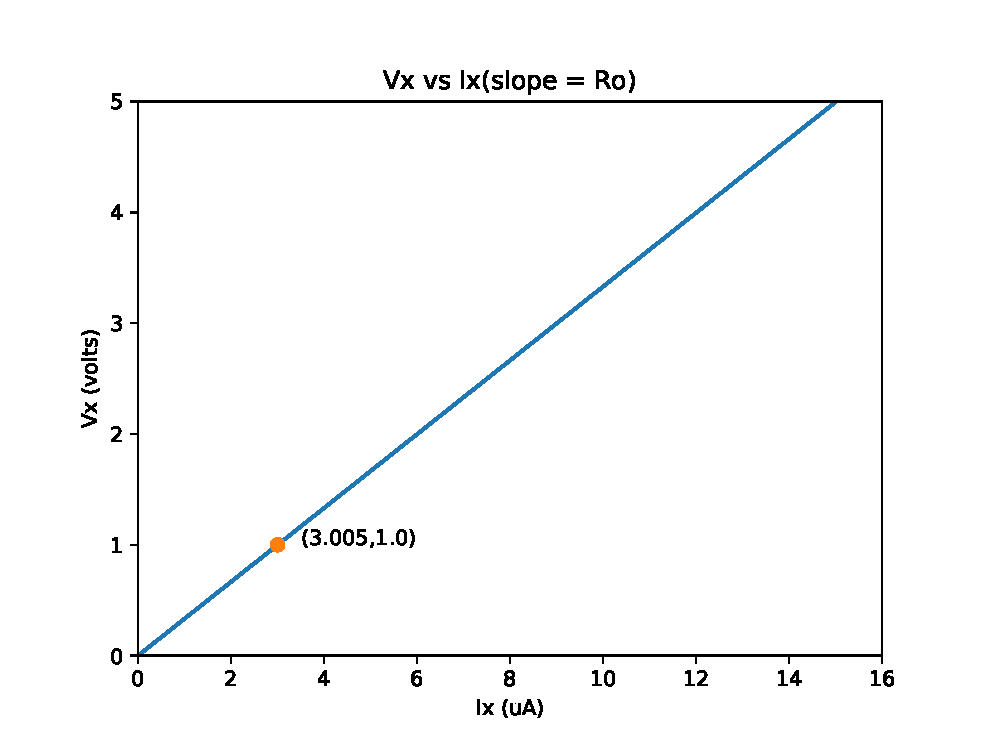
\includegraphics[width=\columnwidth]{./figs/ee18btech11038_rout.eps}
\caption{Simulation for verifying $R_{o}$}
\label{fig:ee18btech11038_rout}
\end{figure}


\item d) To find feedback gain, $H$\\
\solution We know,
\begin{align}
    H = \frac{I_{f}}{I_{0}}, \text{port1 shorted}\\
\end{align}
Therefore,
\begin{align}
    H = \frac{-R_{1}}{R_{1} + R_{2}}
\end{align}

\item e) To find closed-loop gain T\\
\solution 
\begin{align}
    GH = \frac{g_{m1}g_{m2}r_{o1}R_{1}}{g_{m2}(R_{1}||R_{2}) + \frac{R_{1}||R_{2}}{r_{o2}||R_{1}||R_{2}}}
\end{align}
We know, 
\begin{align}
    T = \frac{G}{1+GH}\\ \\
    \implies \frac{-g_{m1}g_{m2}r_{o1}(R_{1} + R_{2})}{g_{m2}(R_{1}||R_{2}) + \frac{R_{1}||R_{2}}{r_{o2}||R_{1}||R_{2}} +g_{m1}g_{m2}r_{o1}R_{1}}
\end{align}

\item Verify the Closed loop gain value.\\
\solution Simulate the circuit, Fig \ref{fig:ee18btech11038_probfig}, using spice. Pass small signal as input $I_{s}$ and observe the output. Fig \ref{fig:ee18btech11038_clgain} shows that $T=-4.96$ which is close to that obtained in Table \ref{table: finalvalues}.
You can find the netlist for the simulated circuit here:
\begin{lstlisting}
spice/ee18btech11038_clgain.cir
\end{lstlisting}
You can find the python script used to generate the output here:
\begin{lstlisting}
spice/ee18btech11038_clgain.py
\end{lstlisting}

\begin{figure}[!ht]
\centering
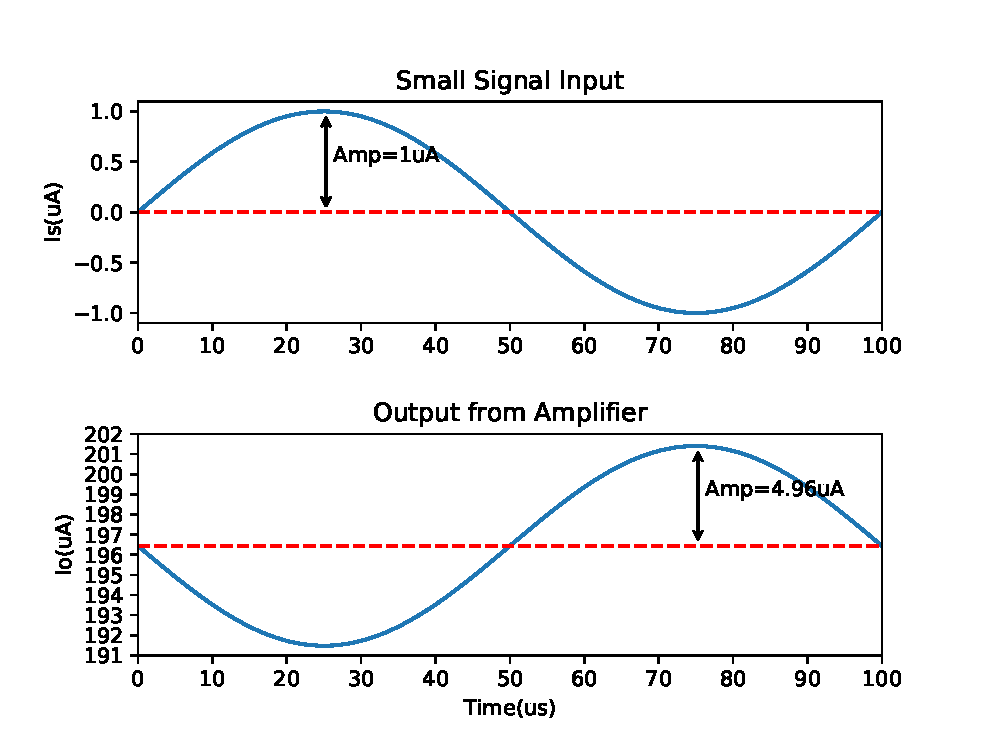
\includegraphics[width=\columnwidth]{./figs/ee18btech11038_clgain.eps}
\caption{Simulation for Closed Loop gain, $T$}
\label{fig:ee18btech11038_clgain}
\end{figure}


\item f) To find $R_{in}$ and $R_{out}$\\
\solution Since $R_{L} =0$ and $R_{s} =\infty$,
\begin{align}
    R_{in} = R_{if} =\frac{R_{i}}{1+GH}
\end{align}
and,
\begin{align}
    R_{out} = R_{of} = (1+GH)R_{o}
\end{align}
Refer \ref{eq:Ri} for $R_{i}$ and \ref{eq:Ro} for $R_{o}$.
Expressions are large for $R_{out}$ and $R_{in}$. Numerical values are calculated in Table \ref{table: finalvalues}.
\begin{table}[!ht]
\centering
%%%%%%%%%%%%%%%%%%%%%%%%%%%%%%%%%%%%%%%%%%%%%%%%%%%%%%%%%%%%%%%%%%%%%%
%%                                                                  %%
%%  This is the header of a LaTeX2e file exported from Gnumeric.    %%
%%                                                                  %%
%%  This file can be compiled as it stands or included in another   %%
%%  LaTeX document. The table is based on the longtable package so  %%
%%  the longtable options (headers, footers...) can be set in the   %%
%%  preamble section below (see PRAMBLE).                           %%
%%                                                                  %%
%%  To include the file in another, the following two lines must be %%
%%  in the including file:                                          %%
%%        \def\inputGnumericTable{}                                 %%
%%  at the beginning of the file and:                               %%
%%        \input{name-of-this-file.tex}                             %%
%%  where the table is to be placed. Note also that the including   %%
%%  file must use the following packages for the table to be        %%
%%  rendered correctly:                                             %%
%%    \usepackage[latin1]{inputenc}                                 %%
%%    \usepackage{color}                                            %%
%%    \usepackage{array}                                            %%
%%    \usepackage{longtable}                                        %%
%%    \usepackage{calc}                                             %%
%%    \usepackage{multirow}                                         %%
%%    \usepackage{hhline}                                           %%
%%    \usepackage{ifthen}                                           %%
%%  optionally (for landscape tables embedded in another document): %%
%%    \usepackage{lscape}                                           %%
%%                                                                  %%
%%%%%%%%%%%%%%%%%%%%%%%%%%%%%%%%%%%%%%%%%%%%%%%%%%%%%%%%%%%%%%%%%%%%%%

 

%%  This section checks if we are begin input into another file or  %%
%%  the file will be compiled alone. First use a macro taken from   %%
%%  the TeXbook ex 7.7 (suggestion of Han-Wen Nienhuys).            %%
\def\ifundefined#1{\expandafter\ifx\csname#1\endcsname\relax}


%%  Check for the \def token for inputed files. If it is not        %%
%%  defined, the file will be processed as a standalone and the     %%
%%  preamble will be used.                                          %%
\ifundefined{inputGnumericTable}

%%  We must be able to close or not the document at the end.        %%
	\def\gnumericTableEnd{\end{document}}


%%%%%%%%%%%%%%%%%%%%%%%%%%%%%%%%%%%%%%%%%%%%%%%%%%%%%%%%%%%%%%%%%%%%%%
%%                                                                  %%
%%  This is the PREAMBLE. Change these values to get the right      %%
%%  paper size and other niceties.                                  %%
%%                                                                  %%
%%%%%%%%%%%%%%%%%%%%%%%%%%%%%%%%%%%%%%%%%%%%%%%%%%%%%%%%%%%%%%%%%%%%%%

	\documentclass[12pt%
			  %,landscape%
                    ]{report}
       \usepackage[latin1]{inputenc}
       \usepackage{fullpage}
       \usepackage{color}
       \usepackage{array}
       \usepackage{longtable}
       \usepackage{calc}
       \usepackage{multirow}
       \usepackage{hhline}
       \usepackage{ifthen}

	


%%  End of the preamble for the standalone. The next section is for %%
%%  documents which are included into other LaTeX2e files.          %%
\else

%%  We are not a stand alone document. For a regular table, we will %%
%%  have no preamble and only define the closing to mean nothing.   %%
    \def\gnumericTableEnd{}

%%  If we want landscape mode in an embedded document, comment out  %%
%%  the line above and uncomment the two below. The table will      %%
%%  begin on a new page and run in landscape mode.                  %%
%       \def\gnumericTableEnd{\end{landscape}}
%       \begin{landscape}


%%  End of the else clause for this file being \input.              %%
\fi

%%%%%%%%%%%%%%%%%%%%%%%%%%%%%%%%%%%%%%%%%%%%%%%%%%%%%%%%%%%%%%%%%%%%%%
%%                                                                  %%
%%  The rest is the gnumeric table, except for the closing          %%
%%  statement. Changes below will alter the table's appearance.     %%
%%                                                                  %%
%%%%%%%%%%%%%%%%%%%%%%%%%%%%%%%%%%%%%%%%%%%%%%%%%%%%%%%%%%%%%%%%%%%%%%

\providecommand{\gnumericmathit}[1]{#1} 
%%  Uncomment the next line if you would like your numbers to be in %%
%%  italics if they are italizised in the gnumeric table.           %%
%\renewcommand{\gnumericmathit}[1]{\mathit{#1}}
\providecommand{\gnumericPB}[1]%
{\let\gnumericTemp=\\#1\let\\=\gnumericTemp\hspace{0pt}}
 \ifundefined{gnumericTableWidthDefined}
        \newlength{\gnumericTableWidth}
        \newlength{\gnumericTableWidthComplete}
        \newlength{\gnumericMultiRowLength}
        \global\def\gnumericTableWidthDefined{}
 \fi
%% The following setting protects this code from babel shorthands.  %%
 \ifthenelse{\isundefined{\languageshorthands}}{}{\languageshorthands{english}}
%%  The default table format retains the relative column widths of  %%
%%  gnumeric. They can easily be changed to c, r or l. In that case %%
%%  you may want to comment out the next line and uncomment the one %%
%%  thereafter                                                      %%
\providecommand\gnumbox{\makebox[0pt]}
%%\providecommand\gnumbox[1][]{\makebox}

%% to adjust positions in multirow situations                       %%
\setlength{\bigstrutjot}{\jot}
\setlength{\extrarowheight}{\doublerulesep}

%%  The \setlongtables command keeps column widths the same across  %%
%%  pages. Simply comment out next line for varying column widths.  %%
\setlongtables

\setlength\gnumericTableWidth{%
	83pt+%
	91pt+%
0pt}
\def\gumericNumCols{2}
\setlength\gnumericTableWidthComplete{\gnumericTableWidth+%
         \tabcolsep*\gumericNumCols*2+\arrayrulewidth*\gumericNumCols}
\ifthenelse{\lengthtest{\gnumericTableWidthComplete > \linewidth}}%
         {\def\gnumericScale{\ratio{\linewidth-%
                        \tabcolsep*\gumericNumCols*2-%
                        \arrayrulewidth*\gumericNumCols}%
{\gnumericTableWidth}}}%
{\def\gnumericScale{1}}

%%%%%%%%%%%%%%%%%%%%%%%%%%%%%%%%%%%%%%%%%%%%%%%%%%%%%%%%%%%%%%%%%%%%%%
%%                                                                  %%
%% The following are the widths of the various columns. We are      %%
%% defining them here because then they are easier to change.       %%
%% Depending on the cell formats we may use them more than once.    %%
%%                                                                  %%
%%%%%%%%%%%%%%%%%%%%%%%%%%%%%%%%%%%%%%%%%%%%%%%%%%%%%%%%%%%%%%%%%%%%%%

\ifthenelse{\isundefined{\gnumericColA}}{\newlength{\gnumericColA}}{}\settowidth{\gnumericColA}{\begin{tabular}{@{}p{83pt*\gnumericScale}@{}}x\end{tabular}}
\ifthenelse{\isundefined{\gnumericColB}}{\newlength{\gnumericColB}}{}\settowidth{\gnumericColB}{\begin{tabular}{@{}p{91pt*\gnumericScale}@{}}x\end{tabular}}

\begin{tabular}[c]{%
	b{\gnumericColA}%
	b{\gnumericColB}%
	}

%%%%%%%%%%%%%%%%%%%%%%%%%%%%%%%%%%%%%%%%%%%%%%%%%%%%%%%%%%%%%%%%%%%%%%
%%  The longtable options. (Caption, headers... see Goosens, p.124) %%
%	\caption{The Table Caption.}             \\	%
% \hline	% Across the top of the table.
%%  The rest of these options are table rows which are placed on    %%
%%  the first, last or every page. Use \multicolumn if you want.    %%

%%  Header for the first page.                                      %%
%	\multicolumn{2}{c}{The First Header} \\ \hline 
%	\multicolumn{1}{c}{colTag}	%Column 1
%	&\multicolumn{1}{c}{colTag}	\\ \hline %Last column
%	\endfirsthead

%%  The running header definition.                                  %%
%	\hline
%	\multicolumn{2}{l}{\ldots\small\slshape continued} \\ \hline
%	\multicolumn{1}{c}{colTag}	%Column 1
%	&\multicolumn{1}{c}{colTag}	\\ \hline %Last column
%	\endhead

%%  The running footer definition.                                  %%
%	\hline
%	\multicolumn{2}{r}{\small\slshape continued\ldots} \\
%	\endfoot

%%  The ending footer definition.                                   %%
%	\multicolumn{2}{c}{That's all folks} \\ \hline 
%	\endlastfoot
%%%%%%%%%%%%%%%%%%%%%%%%%%%%%%%%%%%%%%%%%%%%%%%%%%%%%%%%%%%%%%%%%%%%%%

\hhline{|-|-}
	 \multicolumn{1}{|p{\gnumericColA}|}%
	{\gnumericPB{\raggedright}\gnumbox[l]{\textbf{Parameter}}}
	&\multicolumn{1}{p{\gnumericColA}|}%
	{\gnumericPB{\raggedright}\gnumbox[l]{\textbf{Value}}}
\\
\hhline{|-|-}
	 \multicolumn{1}{|p{\gnumericColA}|}%
	{\gnumericPB{\raggedright}\gnumbox[l]{\textbf{$R_{1}$}}}
	&\multicolumn{1}{p{\gnumericColA}|}%
	{\gnumericPB{\raggedright}\gnumbox[l]{\textbf{$3.5k\Omega$}}}
\\
\hhline{|-|-}
	 \multicolumn{1}{|p{\gnumericColA}|}%
	{\gnumericPB{\raggedright}\gnumbox[l]{\textbf{$R_{2}$}}}
	&\multicolumn{1}{p{\gnumericColA}|}%
	{\gnumericPB{\raggedright}\gnumbox[l]{\textbf{$14k\Omega$}}}
\\
\hhline{|-|-}
	 \multicolumn{1}{|p{\gnumericColA}|}%
	{\gnumericPB{\raggedright}\gnumbox[l]{\textbf{$g_{m1}$}}}
	&\multicolumn{1}{p{\gnumericColA}|}%
	{\gnumericPB{\raggedright}\gnumbox[l]{\textbf{$2mA/V$}}}
\\
\hhline{|-|-}
	 \multicolumn{1}{|p{\gnumericColA}|}%
	{\gnumericPB{\raggedright}\gnumbox[l]{\textbf{$g_{m2}$}}}
	&\multicolumn{1}{p{\gnumericColA}|}%
	{\gnumericPB{\raggedright}\gnumbox[l]{\textbf{$2mA/V$}}}
\\
\hhline{|-|-}
	 \multicolumn{1}{|p{\gnumericColA}|}%
	{\gnumericPB{\raggedright}\gnumbox[l]{\textbf{$r_{o1}$}}}
	&\multicolumn{1}{p{\gnumericColB}|}%
	{\gnumericPB{\raggedright}\gnumbox[l]{\textbf{$50k\Omega$}}}
\\
\hhline{|-|-}
	 \multicolumn{1}{|p{\gnumericColA}|}%
	{\gnumericPB{\raggedright}\gnumbox[l]{\textbf{$r_{o2}$}}}
	&\multicolumn{1}{p{\gnumericColA}|}%
	{\gnumericPB{\raggedright}\gnumbox[l]{\textbf{$50k\Omega$}}}
\\
\hhline{|-|-}
	 \multicolumn{1}{|p{\gnumericColA}|}%
	{\gnumericPB{\raggedright}\gnumbox[l]{\textbf{$R_{s}$}}}
	&\multicolumn{1}{p{\gnumericColA}|}%
	{\gnumericPB{\raggedright}\gnumbox[l]{\textbf{$\infty$}}}
\\
\hhline{|-|-}
	 \multicolumn{1}{|p{\gnumericColA}|}%
	{\gnumericPB{\raggedright}\gnumbox[l]{\textbf{$R_{L}$}}}
	&\multicolumn{1}{p{\gnumericColA}|}%
	{\gnumericPB{\raggedright}\gnumbox[l]{\textbf{$0$}}}
\\

\hhline{|-|-}
	 \multicolumn{1}{|p{\gnumericColA}|}%
	{\gnumericPB{\raggedright}\gnumbox[l]{\textbf{$A$}}}
	&\multicolumn{1}{p{\gnumericColA}|}%
	{\gnumericPB{\raggedright}\gnumbox[l]{\textbf{$-526.3$}}}
\\
\hhline{|-|-}
	 \multicolumn{1}{|p{\gnumericColA}|}%
	{\gnumericPB{\raggedright}\gnumbox[l]{\textbf{$R_{i}$}}}
	&\multicolumn{1}{p{\gnumericColA}|}%
	{\gnumericPB{\raggedright}\gnumbox[l]{\textbf{$17.5k\Omega$}}}
\\
\hhline{|-|-}
	 \multicolumn{1}{|p{\gnumericColA}|}%
	{\gnumericPB{\raggedright}\gnumbox[l]{\textbf{$R_{o}$}}}
	&\multicolumn{1}{p{\gnumericColA}|}%
	{\gnumericPB{\raggedright}\gnumbox[l]{\textbf{$332.8k\Omega$}}}
\\
\hhline{|-|-}
	 \multicolumn{1}{|p{\gnumericColA}|}%
	{\gnumericPB{\raggedright}\gnumbox[l]{\textbf{$\beta$}}}
	&\multicolumn{1}{p{\gnumericColA}|}%
	{\gnumericPB{\raggedright}\gnumbox[l]{\textbf{$-0.2$}}}
\\
\hhline{|-|-}
	 \multicolumn{1}{|p{\gnumericColA}|}%
	{\gnumericPB{\raggedright}\gnumbox[l]{\textbf{$A\beta$}}}
	&\multicolumn{1}{p{\gnumericColA}|}%
	{\gnumericPB{\raggedright}\gnumbox[l]{\textbf{$105.26$}}}
\\
\hhline{|-|-}
	 \multicolumn{1}{|p{\gnumericColA}|}%
	{\gnumericPB{\raggedright}\gnumbox[l]{\textbf{$A_{f}$}}}
	&\multicolumn{1}{p{\gnumericColA}|}%
	{\gnumericPB{\raggedright}\gnumbox[l]{\textbf{$-4.95$}}}
\\
\hhline{|-|-}
	 \multicolumn{1}{|p{\gnumericColA}|}%
	{\gnumericPB{\raggedright}\gnumbox[l]{\textbf{$R_{in}$}}}
	&\multicolumn{1}{p{\gnumericColA}|}%
	{\gnumericPB{\raggedright}\gnumbox[l]{\textbf{$164\Omega$}}}
\\
\hhline{|-|-}
	 \multicolumn{1}{|p{\gnumericColA}|}%
	{\gnumericPB{\raggedright}\gnumbox[l]{\textbf{$R_{out}$}}}
	&\multicolumn{1}{p{\gnumericColA}|}%
	{\gnumericPB{\raggedright}\gnumbox[l]{\textbf{$35.3M\Omega$}}}
\\


\hhline{|-|-|}
\end{tabular}

\ifthenelse{\isundefined{\languageshorthands}}{}{\languageshorthands{\languagename}}
\gnumericTableEnd
\caption{Numerical Values}
\label{table: finalvalues}
\end{table}

\end{enumerate}